\chapter{The CMS experiment at the LHC}
\label{chap:detector}

\chapterquote{Traditional scientific method has always been, at the
very best, 20-20 hindsight. It's good for seeing where you've been.
It's good for testing the truth of what you think you know, but it
can't tell you where you ought to go.}%
{Robert M. Pirsig, Zen and the art of motorcycle maintenance}

The \LHC is one of the largest machines ever built. It exists within a
27~km tunnel $O(100$~m$)$ underground on the border of France and
Switzerland. Along the extent of the \LHC are built a series of
detectors that can record in a high level of detail the result of high
energy particle collisions produced by the collider. This chapter
will focus on the details and performance of \CMS, a multi-purpose
detector optimised to search for new, as yet undiscovered, particles.

\section{The LHC}
\label{sec:lhc}

The \LHC is a hadron collider designed to collide protons and lead
ions at centre of mass energies up to 14\tev, the highest ever achieved by such a
machine
\cite{Evans:2008zzb,CERN-2004-003-V-1,CERN-2004-003-V-2,CERN-2004-003-V-3}.
The proton-proton collisions are most utilised for direct searches for
new physics and therefore take up the vast majority of the \LHC's
running time. 

To bring protons up to the $6.5\tev$ required in Run~2 of the \LHC they are
accelerated through a series of stages. Hydrogen atoms are initially stripped
of their electrons and accelerated to 50\mev by a linear accelerator,
\ac{LINAC2}. The energy is then increased to 1.4\gev by the \ac{PSB} before
being injected into the \ac{PS} which brings the energies up to 26\gev. A final
kick up to 450\gev is provided by the \ac{SPS}. This chain of accelerators also
collect the protons into bunches that are either 25~ns (from Run~2 onwards) or
50~ns apart (during Run~1 and early stages of Run~2). These bunches are then
injected into the \LHC, in which they are steered by around 1200
superconducting dipole magnets while being accelerated up to $6.5\tev$ with
\ac{RF} cavities. Once the beam has reached the intended energy and is stable,
protons are collided at four different points on the ring, around which are
built the four major \LHC detectors, ALICE \cite{Aamodt:2008zz}, ATLAS
\cite{Aad:2008zzm}, LHCb \cite{Alves:2008zz} and \CMS \cite{Chatrchyan:2008aa}.
A representation of this accelerator complex and the location of the
detectors can be seen in Fig.~\ref{fig:lhc}.

\begin{figure}
  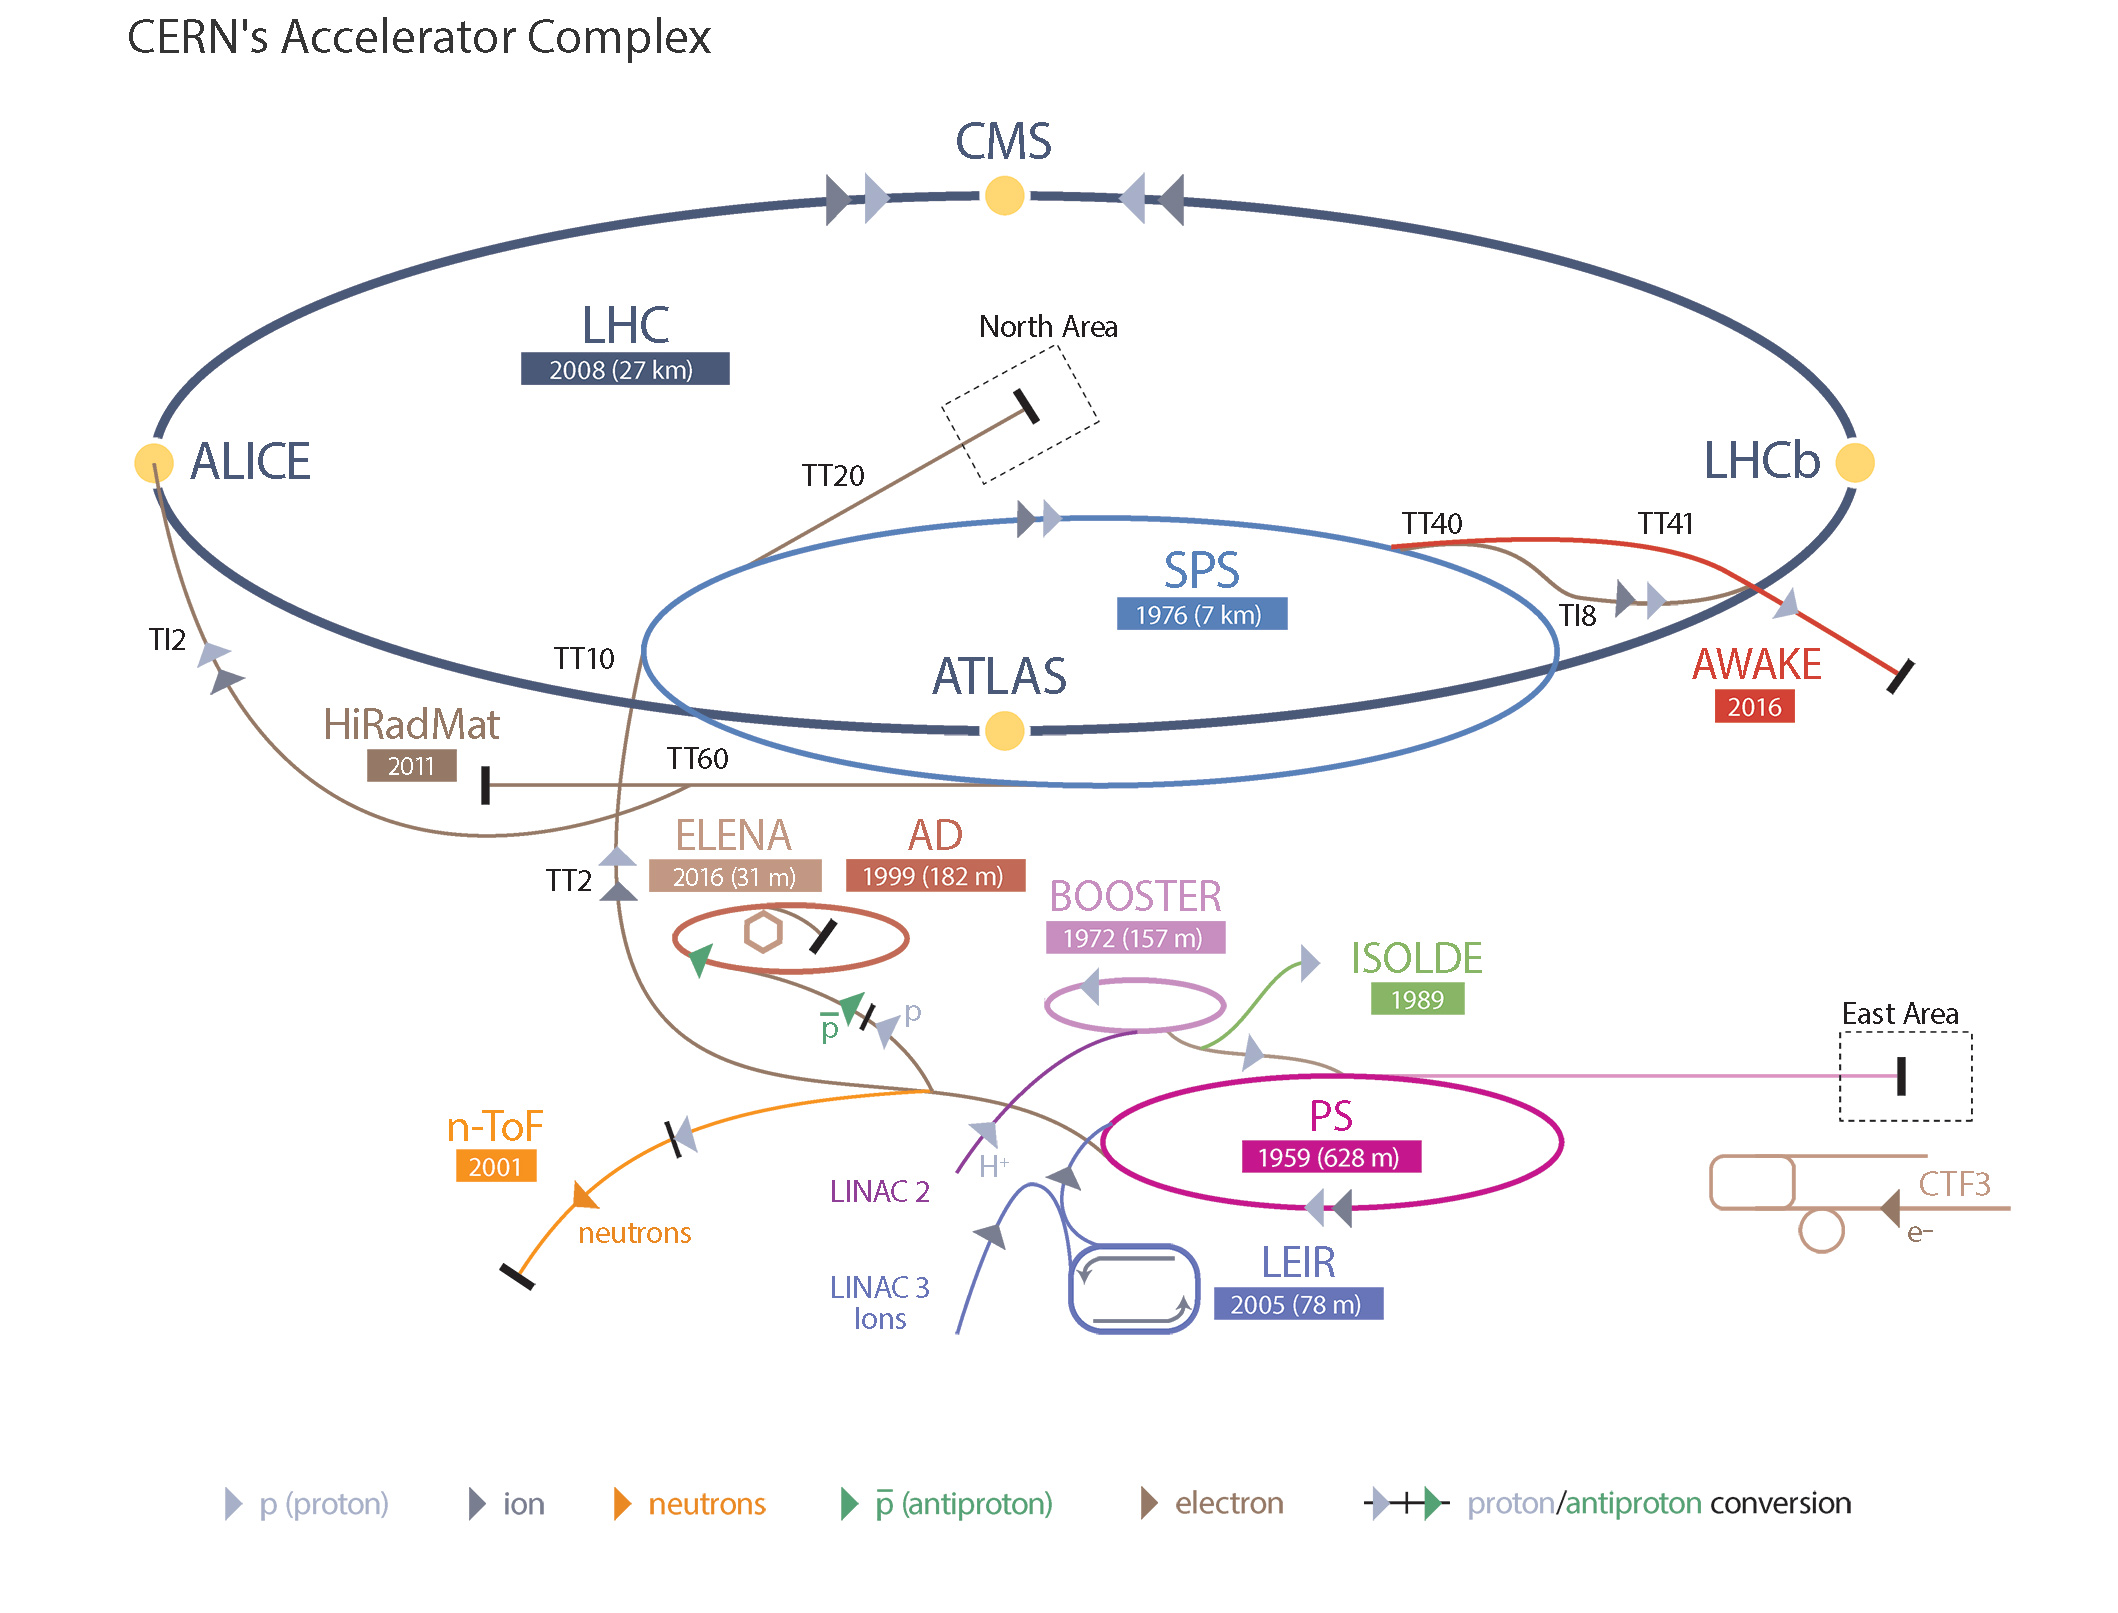
\includegraphics[width=\largefigwidth]{figs/LHC_default}
  \caption[]%
  {A representation of the CERN accelerator complex that help
  accelerate protons to record energies within the \LHC
  \cite{stfc:lhc}}%
  \label{fig:lhc}
\end{figure}

As well as attaining record breaking energies, the \LHC is designed to
collide hadrons at a very high luminosity, with a bunch collision rate
of up to $40~\mhz$ \cite{Evans:2008zzb}. This is necessitated by the
fact that the rate at which electroweak scale processes
occur in proton collisions is significantly lower than their
associated backgrounds, demonstrated in Fig.~\ref{fig:xsecs}.
The \LHC is therefore designed to run at an instantaneous
luminosity approaching $10^{34}$cm$^{-2}$s$^{-1}$ to maximise the occurence of
these rare processes. Along with the high collision rate, this
luminosity is achieved by squeezing the proton bunches to increase the
number of simultaneous collisions per bunch crossing, the extra
simultaneous collisions are known as \PU.  The \LHC has typically
operated with a \PU of $\sim10\mbox{-}20$, however to increase the
luminosity in the future this value will be increased up to a \PU of
O(100).
% , presenting a significant challenge for current and future 
% physics analyses at the \LHC.

\begin{figure}
  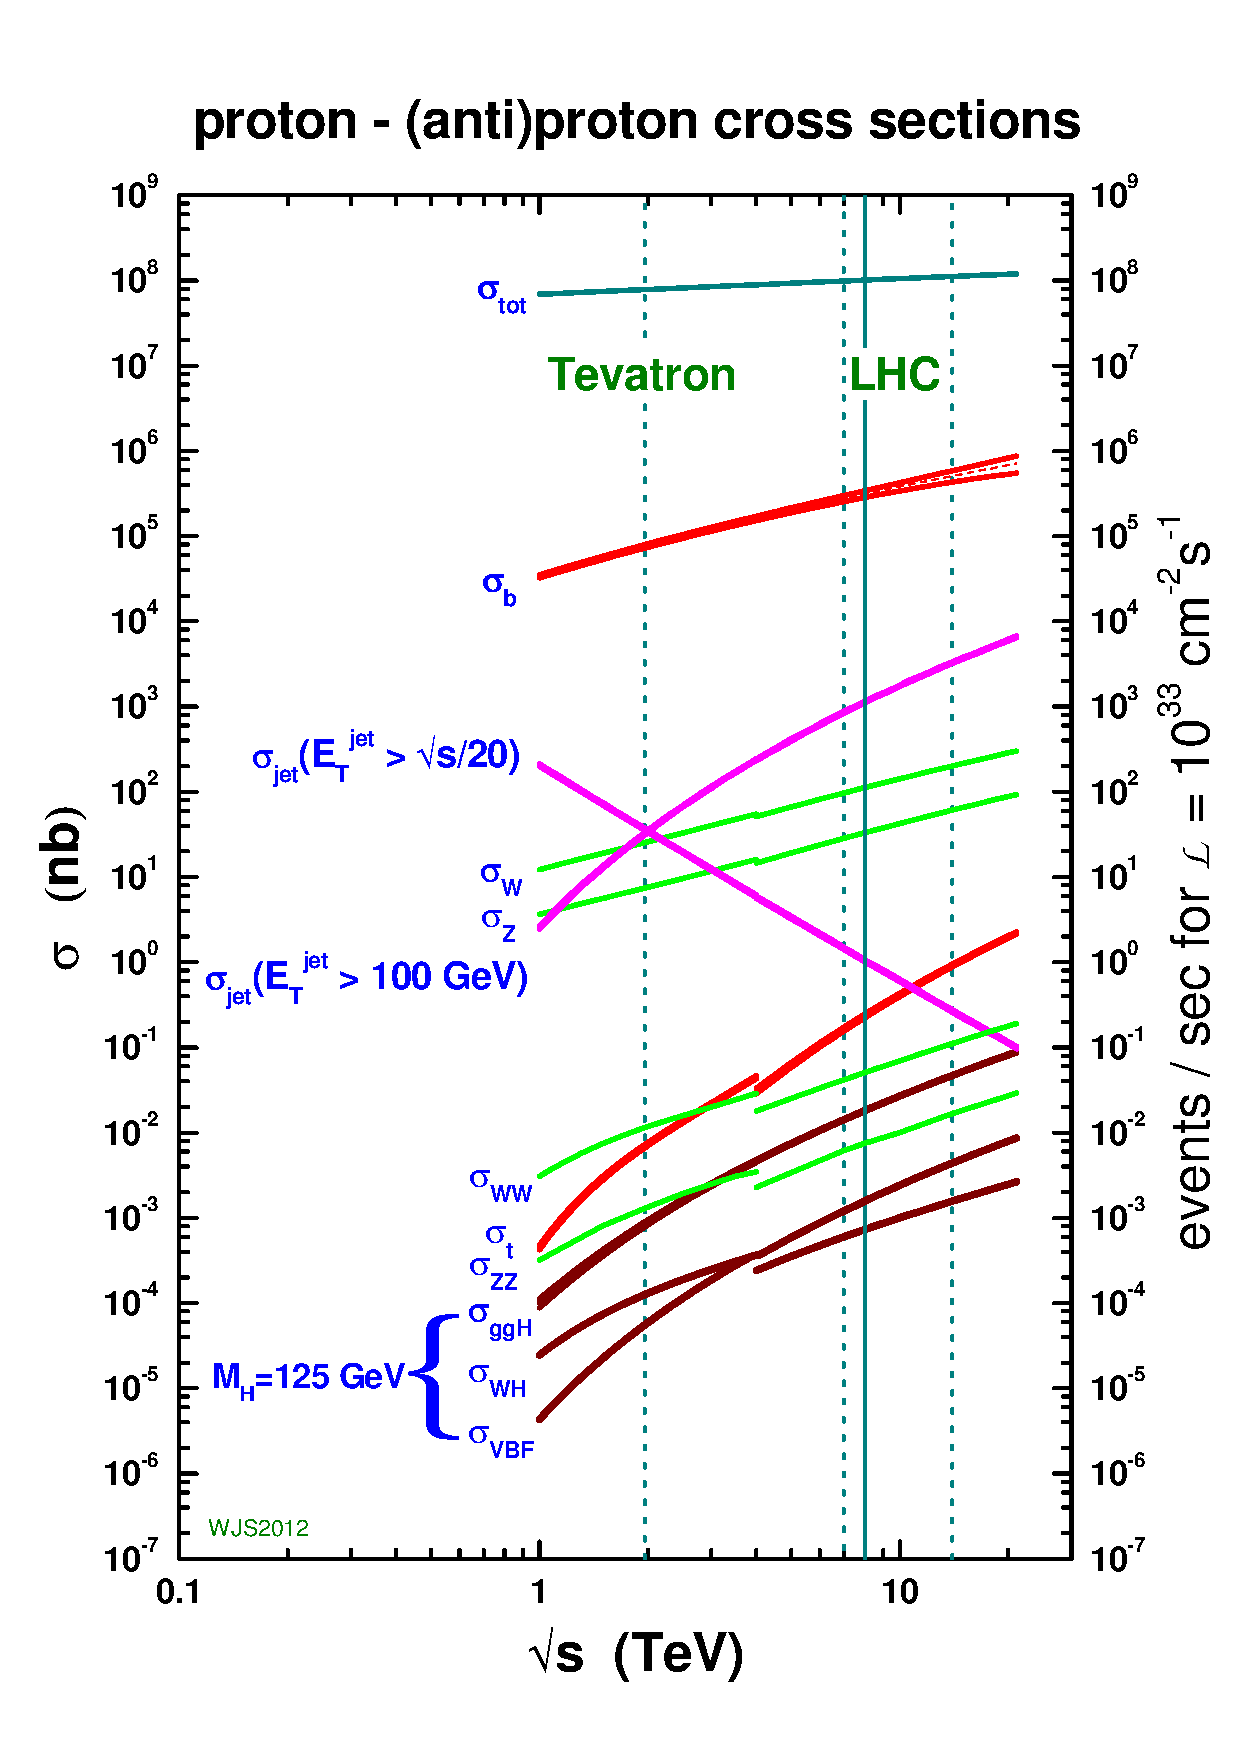
\includegraphics[width=\mediumfigwidth]{figs/crosssections2012_v5}
  \caption[]%
  { The cross sections for various standard model processes as a
  function of proton collider energy, demonstrating the importance of
  high luminosities when observing electroweak scale processes
  \cite{stirlingCrossSec1}.}%
  \label{fig:xsecs}
\end{figure}

During Run~1 of the \LHC, from 2010-2013, a total of $23.3~\ifb$ of
data were collected at centre of mass energies of $\sqrt{s}=7~\tev$ and
$8~\tev$. After this there was a period of shutdown in which the \LHC
and the detectors underwent a series of upgrades. Run~2 then began in
2015 with the collision of protons at $\sqrt{s}=13~\tev$. During 2015 a
total of $4.3~\ifb$ were collected at this energy. So far in 2016 the
\LHC has delivered $34.6~\ifb$, a record breaking number of collisions
at the highest ever recorded energies. 

\section{The CMS detector} \label{sec:cms}

The \CMS detector is one of two multipurpose detectors built around
proton beam collision points, the other being ATLAS. It is situated at
Point 5 on the \LHC, as visibile in Fig.~\ref{fig:lhc}. The key goals
of the \CMS detector at its conception were the discovery of the \SM
Higgs boson and searches for generic signatures of \BSM physics. In \CMS the
results of collisions are measured with a series of subdetectors,
built within and around a $3.8~T$ superconducting solenoid. They are designed to
track, identify and record the energy of all non-neutrino \SM particles
\cite{Bayatian:2006zz}. With its comprehensive, close to $4\pi$, solid
angle coverage, \CMS is well suited to inferring the existence of
weakly interacting particles through the momentum imbalance of visible
particles. This is particularly relevant when searching for \BSM
physics.

\begin{figure}
\begin{center}
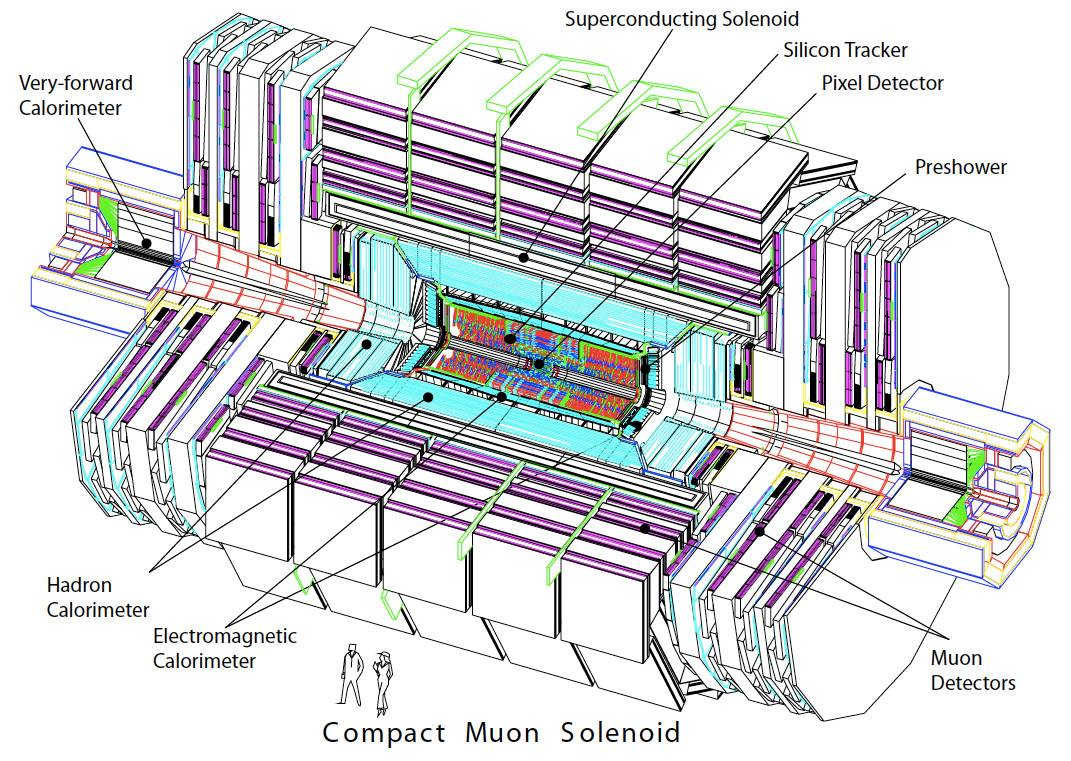
\includegraphics[width=0.8\linewidth]{figs/cms_detector} \end{center}
\caption{An internal view of the Compact Muon Solenoid detector
highlighting the key detecting components \cite{Bayatian:2006zz}}
\label{fig:CMS} \end{figure}

A representative view of \CMS and its components can be seen in
Fig.~\ref{fig:CMS}. The detector is designed in a series of
cylindrical layers of subdetectors working out from the central point,
where the proton collisions occur. The first layer consists of the
silicon tracking system. This tracker is designed to allow the
reconstruction of the trajectory of charged particles produced in the
collision point as they move through the magnetic field. The degree to
which the path of these particles is bent allows for an accurate
determination of their momentum. The next layer beyond the silicon
tracker is the \ECAL, which is designed to absorb and measure the
energy of electrons and photons. Surrounding this is the \HCAL that
absorbs the remaining hadronic particles that have punched through the
\ECAL. Surrounding the tracker and calorimeters is the superconducting
solenoid. In the final layer are the muon chambers and iron return
yoke. The chambers are designed to detect the presence of muons that
will not be absorbed by the central components of the detector. The
data from all these subdetectors are read out by dedicated front end
electronics. It is initially analysed at a basic level by the \CMS
trigger system. The most promising data is then kept and stored for
``offline'' physics analysis. 

Explain the coordinate system..

Explain the pT...

\subsection{The Inner Tracking System} Within the superconducting
solenoid is the silicon tracking system that can track
\mbox{$p_T>1$~GeV} charged particles with an efficiency greater than
$99\%$ \cite{Bayatian:2006zz}.
The Pixel Detector is the high granularity component of the tracking
system that sits closest to the interaction point, covering the
pseudorapidity region $|\eta|<2.1$ \footnote{$\eta \equiv
-ln[tan\frac{\theta}{2}]$, where $\theta$ is measured with respect to
the z-axis that points along the beam direction.}. The Silicon Strip
Tracker sits around this with barrel and endcap components covering
$|\eta|<2.4$. By measuring the curvature of their tracks, charged
particle momenta can be measured with an error between $1.5\%$ and
$3\%$ for $p_T\sim 100$ GeV \cite{Adam_Elwood_MSci}. The resolution of
the trackers is such that the points of origin of event decay products
can be inferred within $10$~$\mu$m, allowing the performance of CMS to
extend up to very high pileup (number of simultaneous collisions)
\cite{CMSTrackPerformance}.

\subsection{The Electromagnetic and Hadronic Calorimeters} Surrounding
the tracking system are the electromagnetic and hadronic calorimeters
(\ECAL and \HCAL). The \ECAL is constructed from 75~848 PbWO$_4$
scintillating crystals covering $|\eta|<3$. They are designed to
absorb electrons and photons and emit light proportional to the energy
deposited. This light is detected by custom photodiodes designed to
perform well in high magnetic fields.  \\\\ The \HCAL is designed to
absorb hadrons and is constructed from brass absorbers interleaved
with scintillating plastic tiles covering $|\eta|<3$. The
scintillations are read out with hybrid photodiodes via wavelength
shifting fibres.  \\\\ In the forward detector regions, the hadronic
calorimetry is extended up to $|\eta|<5$ with the Forward Calorimeter,
made from steel absorber with quartz scintillating fibre. To also help
prevent signal contamination from low energy neutral pions there is a
Preshower detector consisting of lead absorbers and silicon
microstrips \cite{CMSTechDesign1DetectorPerformance}\cite{Cutajar}.

\subsection{The Muon System} As muons are unlikely to be absorbed in
the \ECAL and \HCAL, a muon system is built into the iron return yoke
that surrounds the solenoid.  This consists of wire chambers
containing ionising gas that allows the measurement of muon momenta
with a greater than $1\%$ precision
\cite{CMS_Overview_Chatrchyan:2008aa}.

\subsection{The Trigger and Data Acquisition System}
\label{sec:triggers} The rate of collisions at the LHC is so high that
it would be impossible to reconstruct and store the results of all
collision events. As the majority of the collisions are soft QCD
processes, they are not useful in the search for new physics at the
electroweak energy scale. This necessitates a multi-level trigger
system that is designed to pick out and store only high centre-of-mass
physics processes. The Level 1 Trigger (L1T) is the first component of
the trigger system and is made from custom FPGA computational boards
situated close to the detector. This uses coarse information from the
calorimeters and muon system to reduce the event rate from $20$MHz
(during Run 1) to $\sim100$kHz. The data from the subdetectors are
then passed to the High Level Trigger (HLT), which uses full detector
information to reconstruct the events and reduce the data rate to
$\sim1$kHz. The remaining events are then fully reconstructed and
stored at various Grid sites \cite{GridTechDesign}.


